%%%%%%%%%%%%%%%%%%%%%%%%%%%%%%%%%%%%%%%%%%%%%%%%%
%%%%%%%%%%%%%%%%%%%%%%%%%%%%%%%%%%%%%%%%%%%%%%%%%

\chapter{Nature Inspired Algorithms for Prioritized Foraging}
\label{chap:third}

%%%%%%%%%%%%%%%%%%%%%%%%%%%%%%%%%%%%%%%%%%%%%%%%%
%%%%%%%%%%%%%%%%%%%%%%%%%%%%%%%%%%%%%%%%%%%%%%%%%

This chapter presents a foraging variation known as prioritized foraging as well as three algorithms whose performance is to be evaluated on a prioritized foraging problem. The three algorithms are based based upon phenomena observed in nature. The first model is a simple foraging algorithm, called Na\"ive foraging, which will form the benchmark algorithm for the experiments. Two novel swarm robotics foraging algorithms, inspired by the foraging behaviour of desert ants and honey bees, are also presented. Each of these algorithms have different capabilities when it comes to memory, communication, division of labour, and navigation. The Na\"ive foraging algorithm is presented in Section~\ref{naiveforaging}. Section~\ref{desertantforaging} introduces the novel foraging algorithm based on desert ants. Section~\ref{honeybeeforaging} presents a novel prioritized foraging algorithm inspired by honey bees. The algorithms are summarized in Section~\ref{prioritized:summary}.
%%%%%%%%%%%%%%%%%%%%%%%%%%%%%%%%%%%%%%%%%%%%%%%%%
%%%%%%%%%%%%%%%%%%%%%%%%%%%%%%%%%%%%%%%%%%%%%%%%%

\section{Prioritized Foraging}
\label{sec:second:prioritizedforaging}

%Focus on the robots used, the model used and the experiments performed

The prioritized foraging problem, illustrated in Fig.\ref{prioritizedforaging}, is a modified version of the multi-foraging problem as discussed in Section~\ref{environmentaxis}. In prioritized foraging, an environment has two types of items: prioritized items and non-prioritized items. The goal is to forage all the items of the prioritized type. The possibility exists that prioritized items become trapped among non-prioritized items and thus the non-prioritized items need to be removed from the environment to clear an access route to the prioritized items. 

The prioritized foraging problem has increased difficulty compared to traditional multi-foraging problems, due the fact that foraging the non-prioritized item more than required will result in a waste of time and energy. The goal of research in prioritized foraging is to develop an algorithm to efficiently adapt the number of robots searching for prioritized items to those moving non-prioritized items out the way. 

The prioritized foraging problem has similarities to the problem of search and rescue. For example, in the case of a building collapsed, robots will need to get to the survivors as quickly as possible. However, it is important that some robots move waste material in order to reach the priority trapped survivors. Prioritized foraging could be applied to the gold mining problem where gold needs to be foraged as a priority, and waste needs to be moved out of the way.


\begin{figure} [h]
	\centering
	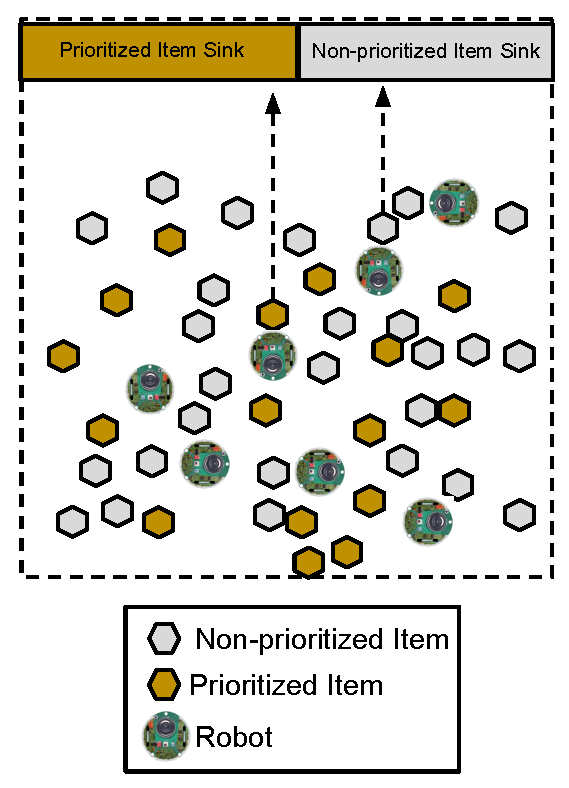
\includegraphics[width=0.65\textwidth]{chapters/chapter2/figures/EpuckGoldMining.pdf}
	\caption{Prioritized Foraging Problem }
	\label{prioritizedforaging}
\end{figure}

As per Winfield's classification discussed in Section~\ref{sec:second:taxonomy}, the prioritized foraging problem has the following characteristics: The environment has a bounded search space, with multiple source areas for items which can be placed in multiple sinks. Multiple object types exist in the environment - the prioritized items and the non-prioritized items. The primary  performance measure for the prioritized foraging problem is time, in terms optimizing the time taken to forage each type of item. 


\section{Na\"ive Foraging Algorithm}
\label{naiveforaging}

 Na\"\i ve foraging consists of the following tasks: searching for an item, grabbing an item, returning home with the item, and storing the item at the sink. The steps performed by the algorithm are illustrated in Figure~\ref{naiveforagingstatediagram}, and described below:  

\begin{enumerate}
	\item Robots perform a random walk until they find an item.
	\item On locating an item, the robot grips the item. If the item has been moved before the robot is able to pick it up, the robot will continue to explore; otherwise, the robot returns the item to the correct sink using a beacon-based homing algorithm.
\end{enumerate}

\begin{figure} [h]
	\centering
	\begin{tikzpicture}[node distance=8cm]
	\node (randomwalk) [process] {random walk};
	\node (offload) [process, below of=randomwalk, yshift=4cm] {off-load};
	\node (loaditem) [process, right of=randomwalk] {load item};
	\node (homing) [process, right of=offload] {homing};
	\draw [arrow] (randomwalk) -- node[anchor=south] {locates item} (loaditem);
	\draw [arrow] (loaditem) -- node[anchor=west] {successful load} (homing);
	\draw [arrow] (homing) -- node[anchor=north] {at sink} (offload);
	\draw [arrow] (offload) -- node[anchor=west] {successful offload} (randomwalk);

	\draw[arrow,postaction={decorate,decoration={text along path,reverse path,raise=1ex,text align=center,text={unsuccessful load}}}] (loaditem) to[bend right=45] (randomwalk);
	\end{tikzpicture}
	\caption{Nai\"ve Foraging State Diagram}
	\label{naiveforagingstatediagram}
\end{figure}

Na\"\i ve foraging includes only the most minimal set of foraging actions and is included as a baseline for comparison to evaluate how novel techniques, such as the desert-ant foraging or honey-bee foraging, compare to a standard model \cite{ostergaard2001emergent,hoff2010two}.

The following random walk is used: A robot chooses a random direction, $\sigma$, and a random distance $m\in(0,M)$ where $M$ is a chosen maximum path length. The robot walks in direction $\sigma$ for distance $m$, or until the robot reaches a boundary. The robot then chooses new values for $\sigma$ and $m$.


\section{Desert Ant Foraging}
\label{desertantforaging}


As discussed in Section~\ref{biological:ants}, desert ant foraging behaviour is a very suitable model for robot foraging, since no pheromone depositors or pheromone mimickry is required. Pheromone depositors or pheromone mimickry are quite complex to perform in robot environments. Instead of pheromone, desert ants use path integration (PI) to memorize the location of an existing food source and later to return to the memorized source to find more food, as discussed in Section~\ref{biological:ants}. The notion of returning to a previously explored site is known as site fidelity \cite{switzer1993site}. The desert ant algorithm does not require communication between robots or the dispersal of beacons, and is thus simpler than many other swarm robotic foraging algorithms. The desert ant foraging robots can be in the following states:

\begin{enumerate}
	\item\textbf{Exploration State}: A robot in the exploration state performs a random walk with PI. The random walk used is the same random walk as discussed in Section~\ref{naiveforaging}. The purpose of the exploration state is to explore the environment to locate items. 
	\item\textbf{Loading State}: On finding an item, the robot switches into the loading state. In the loading state, the robot loads the item and memorizes the current PI vector. The PI vector is memorized so that the robot can use it to return to the sink and then later to return to the site where the item was found. If loading of the item fails (perhaps due to another robot loading the item), then the robot returns to the exploration state; otherwise, the robot moves into the homing state.
	\item\textbf{Homing State}: In the homing state, the robot uses the PI vector to move to the sink. The use of the PI vector will enable the robot to follow the most direct route back to the sink.
	\item\textbf{Offloading State}: When the robot arrives at the sink, the robot switches into the offloading state, where the robot simply offloads the item into the sink. 
	\item\textbf{Locating State}: Once the robot has offloaded the item, the robot switches to the locating state. In the locating state, the robot follows the memorized PI vector to the location of the previous item. The premise of returning to the site where the previous item was found is that more items may exist where the previous item was located in order to locate more items. If another item is found, the robot moves into the loading state; otherwise, the robot returns to the exploration state in the search of new items. 
\end{enumerate}

All robots begin at random positions adjacent to the sink in the exploration state. The desert ant foraging states and transitions are illustrated in Figure~\ref{fig:desertantstate}.

\begin{figure} [h]
	\centering
	\begin{tikzpicture}[node distance=6cm]
	\node (explorationstate) [process] {explore};
	\node (loadstate) [process, right of=randomwalk] {loading};
	\node (homing) [process, below of=loadstate,yshift=2cm] {homing};
	\node (offload) [process, left of=homing] {offload};
	\node (locating) [process, left of=explorationstate] {locating};
	\draw [arrow] (explorationstate) -- node[anchor=south] {locates item} (loadstate);
	\draw [arrow] (loadstate) -- node[anchor=west] {successful load} (homing);
	\draw [arrow] (homing) -- node[anchor=south] {at sink} (offload);
	\draw [arrow] (offload) -- node[anchor=east] {offload complete} (locating);
	\draw [arrow] (locating) -- node[anchor=south] {item not found} (explorationstate);
	\draw[arrow,postaction={decorate,decoration={text along path,raise=1ex,text align=center,text={locates item}}}] (locating) to[bend left=45] (loadstate);
	\draw[arrow,postaction={decorate,decoration={text along path,reverse path, raise=1ex,text align=center,text={unsuccessful load}}}] (loadstate) to[bend left=45] (explorationstate);
	\end{tikzpicture}
	\caption{Desert Ant Foraging State Diagram}
	\label{fig:desertantstate}
\end{figure}

	
%%%%%%%%%%%%%%%%%%%%%%%%%%%%%%%%%%%%%%%%%%%%%%%%%
%%%%%%%%%%%%%%%%%%%%%%%%%%%%%%%%%%%%%%%%%%%%%%%%%

\section{Honey Bee Foraging}
\label{honeybeeforaging}
%TODO Describe the 3 states referring back to where they were discussed in the previous section.

Honey bee prioritized foraging algorithm presented in this section is based on the foraging behaviour of honey bees as described in Section~\ref{bees:biologicalinspiration}. The algorithm described requires robots to take on one of three roles, namely, scout robots, unemployed forager robots or employed forager robots. The roles of the robots and the transitions to and from these roles are described in this section. 

Figure~\ref{honeybeestate} provides a simplified diagram for the honey bee prioritized foraging algorithm showing the roles and the transitions between each role and the states within these roles. The dance and explore states of the scout robots are shown separately for clarity and the employed forager states are outlined separately in Figure~\ref{employedforagerstatediagram}.

To more succinctly define the honey bee prioritized foraging algorithm, the algorithms for each behavioural state, within each role, are provided below. For each algorithm, note that the current state of the robot is denoted $state$, and the $state$ is modified during the behaviour to denote the next state of the robot. The current time step is denoted as $t$. The algorithm for a single state is executed once per time step $t$.

\begin{figure}[h]
	\centering
	\begin{tikzpicture}[node distance=10cm]
	\node (wait) [process] {unemployed forager};
	\node (forage) [process, right of=wait] {employed forager};
	\node (dance) [process, below of=forage,yshift=5cm] {dance};
	\node (scout) [process, left of=dance] {explore};
	
	\draw [arrow,postaction={decorate,decoration={text along path,raise=1ex,text align=center,text={recruited}}}] (wait) to[bend left=20] (forage);
	
	\draw [arrow] (forage) -- node[anchor=north] {$i_{forage} \geq t_{forage}$} (wait);
	
	\draw [arrow] (forage) to[bend left=20] node[anchor=west] {$\mu_\varsigma \geq \Phi$} (dance);
	\draw[arrow] (dance) to[bend left=20] node[anchor=east] {$\varrho \geq \rho$} (forage);
	\draw [arrow] (dance) -- node[anchor=south] {$\varrho < \rho$} (scout);
	\draw [arrow] (scout) -- node[anchor=east] {$i_{wait} > t_{wait}$} (wait);
	\draw [arrow,postaction={decorate,decoration={text along path,raise=1ex,text align=center,text={locates new site}}}] (scout) to[bend left=20] (dance);
	\draw [arrow] (forage) to[loop] node[anchor=south] {$\mu_\varsigma < \Phi$} (forage);
	\draw [arrow] (wait) to[loop] node[anchor=south] {$i_{forage} < t_{forage}$} (wait);
	\node[process, fit=(scout)(dance), inner sep=1.5cm, label={270:scout}] (all) {};
	\end{tikzpicture}
	\caption{Honey Bee Foraging State Diagram}
	\label{honeybeestate}
\end{figure}

Section~\ref{scoutrobots} presents the behaviour of scout robots, while the behaviour of forager robots is described in Section~\ref{foragerrobots}. The initial state of the swarm is described in Section~\ref{initialstates}, while Section~\ref{honeybeedivisionoflabour} describes the division of labour mechanism used by the honey bee algorithm.

\subsection{Scout Robots}
\label{scoutrobots}
Scout robots mimic the scouting behaviour of the scout honeys bees as discussed in Section~\ref{bees:biologicalinspiration}. The purpose of the scout robot is to locate sites of items. If the discovered site is of a high enough quality, then the scout will broadcast the location of the site to the unemployed forager robots at the sink. 

Each scout robot begins in the explore state where the scout robot performs a random walk. Algorithm~\ref{algorithm:explore} provides a step-by-step explanation of the explore state of the scout root. Variable $\varsigma$ saves the robot's item specialization. The random walk performed is the same random walk as discussed in Section~\ref{naiveforaging}. As the scout robot moves, the robot maintains a PI vector $v$ as explained in Section~\ref{biological:ants}. Upon finding an item $\vartheta$ of type $\varsigma$ at site $\xi$, the robot loads the item and then performs an evaluation of the quality, $mu_\varsigma$, of the site $\xi$ for the item type $\varsigma$. 


% Scout algorithms
\begin{algorithm}
\caption{Explore State of Scout Robot}
\label{algorithm:explore}
\begin{algorithmic}[1]
\Function{explore}{$role, state, v, \varsigma, i$}
%move random direction from location l
\State \text{perform a random walk step from location}
\State \text{update path integration vector \={$v$}}

\If {\text{item $\vartheta$ of priority $\varsigma$ is detected in vicinity}}
 	\State \text{calculate quality $\mu_\varsigma$ of site $\xi$ }
	\State {$\omega \gets v$}
	\State load item $\vartheta$
\ElsIf {$i_{explore} > f_{max}$ and $i_{explore} \leq t_{explore}$}
	\State $\varsigma \gets N$
\ElsIf {$i_{explore} > t_{explore}$}
	\State $state \gets homing$
\EndIf
\State $i =i + 1$
\EndFunction
\end{algorithmic}
\end{algorithm}

The quality, $\mu_\varsigma$, of site $\xi$, for a robot scouting items of type $\varsigma$ is calculated as the estimated density of items of type $\varsigma$ in the local vicinity of the found item $\vartheta$. The robot has distance sensor values $k_j\in[0,1]$ for $j = 1...n$ where $n$ is the number of distance sensors. A distance sensor reading of 0 means that nothing is detected in the sensor's range and a distance sensor reading of 1 indicates that the robot is touching an item. The sensor value $k_j$, for item type $\varsigma$, denoted $k_{j_\varsigma}$, is calculated as 
\begin{equation}
\label{densitytype}
k_{j_\varsigma}=
    \begin{cases}
      k_j & \text{if detected item is type $\varsigma$} \\
      0 & \text{otherwise}
    \end{cases}
\end{equation}

The site quality of type $\varsigma$, $\mu_\varsigma$, is calculated using
\begin{equation}
\label{density}
\mu_\sigma = \frac{1}{n}\sum\limits_{i=1}^n k_{i_\varsigma}
\end{equation}
 
Before returning to the sink with the item, the scout memorizes the PI vector $v$ in site location variable $\omega$. The scout robot then switches to the homing state as shown in Algorithm~\ref{algorithm:scout:homing}. Using PI vector $\omega$, the scout returns the item $\vartheta$ to the sink. When the scout robot has returned to the sink, $S_\varsigma$, the scout robot offloads the item $\vartheta$. If the quality $\mu_\varsigma$ of the visited site $\xi$ is larger than threshold $\Phi$, the scout robot switches into the dance state, which is depicted in Algorithm~\ref{algorithm:recruit}. If the quality $\mu_\varsigma$ of the visited site $\xi$ is less than threshold $\Phi$, the robot takes on the role of an employed forager and switches into the locate state which is outlined in Algorithm~\ref{algorithm:employedforager:locating}.


\begin{algorithm}
\caption{Homing State of Scout Robot}
\label{algorithm:scout:homing}
\begin{algorithmic}[1]
\Function{scout homing}{$role, state, v, \varsigma, i, \omega$}
\If {\text{robot is at sink $S_\varsigma$ and robot is loaded}}
	\State \text{robot offloads item $\vartheta$}
	\If {\text{$\mu_\varsigma > \phi \text{and} \varsigma = P$}}
		\State \text{$state \gets dance$}
	\Else 
		\State \text{$role \gets \text{employed forager}$}
		\State \text{$state \gets locate$}
	\EndIf
\Else
	\State{\text{calculate direction $d$ to sink $S_\varsigma$ from current location}}
	\If{\text{robot can move in direction $d$}}
		\State \text{robot moves in direction $d$}
	\EndIf
\EndIf
\State $i =i + 1$
\EndFunction
\end{algorithmic}
\end{algorithm}


\begin{algorithm}
\caption{Dance State of Scout Robot}
\label{algorithm:recruit}
\begin{algorithmic}[1]
\Function{dance}{$role, state, v, \varsigma, i, \omega, \mu_\varsigma$}
\If {$i_{dance} < t_{dance}$}
	\State \text{broadcast $\omega$ and $\mu_\varsigma$ to robots at the sink} 
\Else 
	\State \text{$\varrho = random(0,1)$}
	\If {$\varrho < \rho$} 
		\State{$role \gets \text{employed forager}$}
		\State{$state \gets locate$}
	\Else
		\State{$state \gets explore$}
	\EndIf
\EndIf
\State $i =i + 1$
\EndFunction
\end{algorithmic}
\end{algorithm}

% Employed Forager
\begin{algorithm}
\caption{Locate State of Employed Forager}
\label{algorithm:employedforager:locating}
\begin{algorithmic}[1]
\Function{forage}{$role, state, v, \varsigma, i, \omega, \mu_\varsigma$}
	\State \text{direction $d = \omega - l$ }
	\State \text{robot moves in direction $d$}
	\If {\text{$\omega - l == 0$ OR robot can see item of type $\varsigma$}}
		\State $state \gets load$
	\EndIf
	\State $i =i + 1$
\EndFunction
\end{algorithmic}
\end{algorithm}

In the dance state, the scout robot communicates the location, $\omega$, and quality $\mu_\varsigma$, of the previous site $\xi$, to the unemployed workers at the sink. The communication is akin to the waggle dance performed by honey bees in nature, as discussed in Section~\ref{bees:biologicalinspiration}. A scout robot's ``dance" takes the form of a localized broadcast communication between the scout and the unemployed forager robots near the sinks. The scout robot will communicate the site quality and location for the unemployed foragers for $t_{dance}$ time steps.

After the scout robot has completed broadcasting site details to the unemployed foragers, the scout robot must decide to either stay a scout robot and switch back to the explore state or become an employed forager robot and begin foraging the previous site. The scout robot becomes an employed forager robot with the probability of $\rho$. If random number $\varrho\in{0,1}$ is selected such that $\varrho$ is less than $\rho$, then the scout robot remains a scout and begins to explore the environment. If $\varrho$ is greater than or equal to $\rho$ then the scout becomes an employed forager. Increasing the site quality threshold $\rho$ will make the scout robots more selective about the sites they broadcast. Decreasing $\rho$ will result in scout robots being less selective about the sites they broadcast.

\subsection{Forager Robots}
\label{foragerrobots}

There are two types of forager robots: The unemployed foragers and employed foragers. The unemployed forager robots take on the role of unemployed foragers from foraging honey bees discussed in Section~\ref{bees:biologicalinspiration}. Unemployed forager robots remain at the sink and await dance behaviour from a scout robot. This wait state is described in Algorithm~\ref{algorithm:unemployedforager:locating}.

\begin{algorithm}
\caption{Wait State of Unemployed Forager}
\label{algorithm:unemployedforager:locating}
\begin{algorithmic}[1]
\Function{wait}{$state, v, \varsigma, i, \omega, \mu_\varsigma$}
\If {$i_{wait} \geq t_{wait}$}
	\State{$role \gets scout$}
	\State $\varsigma \gets P$
	\State{$state \gets explore$}
\ElsIf {\text{scout robot is broadcasting at sink}}
	\State \text{receive site location $\omega$ and site quality $\mu_\varsigma$}
	\State $role \gets \text{employed forager}$
	\State $state \gets locate$
\EndIf
\State $i =i + 1$
\EndFunction
\end{algorithmic}
\end{algorithm}

When a scout robot dances at the sink after locating an item $\vartheta$, each unemployed forager chooses whether to listen to the details communicated by the scout robot, of the site $\xi$ with a probability $\alpha$. An unemployed forager's acceptance of the site details, that are communicated by a scout robot, is known as recruitment. If an unemployed forager robot is recruited by the scout robot, the unemployed forager robot becomes an employed forager robot. The unemployed forager takes on the same item specialization, $\varsigma$ as the dancing scout robot. The unemployed forager will thus only search for items of type $\varsigma$. 

The employed forager robots are modelled after the employed forager bees as discussed in Section~\ref{bees:biologicalinspiration}. The purpose of the employed forager robot is to forage the sites communicated by scout robots. When an unemployed forager robot takes on the role of an employed forager robot after recruitment by a scout robot, the employed forager starts in the locate state, described in Algorithm~\ref{algorithm:employedforager:locating}. In the locate state, the employed forager robot uses the PI vector $\omega$ to relocate the site $\xi$. Once the site $\xi$ has been relocated, the employed forager robot switches into the load state has been described in Algorithm~\ref{algorithm:loading}. If an item $\vartheta$ of type $\varsigma$ is detected in the vicinity of the located site, then the item is loaded. After successfully loading the item, the robot switches to the homing state. If the employed forager robot does not detect an object in the vicinity of the site $\xi$, then the employed robot switches to the local search state in order to perform a brief local search for items nearby. 

\begin{algorithm}
\caption{Load State of Employed Forager}
\label{algorithm:loading}
\begin{algorithmic}[1]
\Function{loading}{$role, state, v, \varsigma, i, \omega, \mu_\varsigma$}
\If {\text{item $\vartheta$ of priority $\varsigma$ is detected in vicinity}}
	\State \Call{load}{$\vartheta$}
	\State{$state \gets homing$}
\Else
	\State{$state \gets local\_search$}
\EndIf
\EndFunction
\end{algorithmic}
\end{algorithm}

The local search is performed for a limited number of time steps $t_{ls}$. At each time step $i_{ls}$, the robot checks if an item of priority $\varsigma$ is nearby and can be loaded. If an item $\varsigma$ can be loaded then the robot loads the item and switches to the homing state. If the employed forager robot can see an item $\varsigma$, but it is not close enough to be loaded, then the robot moves in the direction of the item $\varsigma$. If the employed forager can't see an item in the vicinity, then the robot moves in a random direction $d$. Local search state is shown in Algorithm~\ref{algorithm:employedforager:localclustersearch}. If $i_{ls}$ is greater than $t_{ls}$, then the foraging site is depleted and so the employed forager robot must return to the sink without an item.

\begin{algorithm}
\caption{Local Search State of Employed Forager}
\label{algorithm:employedforager:localclustersearch}
\begin{algorithmic}[1]
\Function{local\_search}{$role, state, v, \varsigma, i, \omega, \mu_\varsigma$}
\If {\text{$i_{ls} < t_{ls}$}}
		\If {\text{item $\vartheta$ of priority $\varsigma$ is nearby and can be loaded}}
			\State \Call{load}{$\vartheta$}
			\State{$state \gets homing$}	
		\ElsIf {\text{item $\vartheta$ of priority $\varsigma$ can be seen but is not close enough}}
			\State \text{select direction $d$ to move towards item $\vartheta$}
			\State \text{robot moves in direction $d$}
		\Else
			\State \text{select a random direction $d$}
			\State \text{robot moves in direction $d$}	
		\EndIf
\Else
	\State{$state \gets homing$}
\EndIf
\State $i =i + 1$
\EndFunction
\end{algorithmic}
\end{algorithm}

When in the homing state, the employed forager robot moves towards the appropriate sink $S_\varsigma$ in order to off-load item $\vartheta$. Once at sink $S_\varsigma$, if the employed forager robot is loaded, it offloads the item and switches back to the locate state and thus repeats the steps of foraging the site $\xi$. If the employed forager robot is not loaded, the employed forager robot takes on the role of an unemployed forager and switches into the wait state. The reason for switching from an employed forager to an unemployed forager is because an item could not be found at the site $\xi$ and thus the site has likely been depleted so the employed forager switches to an unemployed forager in order to await recruitment by a scout robot.

\begin{algorithm}
\caption{Homing State of Employed Forager Robot}
\label{algorithm:forager:homing}
\begin{algorithmic}[1]
\Function{employed forager homing}{$role, state, v, \varsigma, i, \omega$}
\If {\text{robot is at sink $S_\varsigma$}}
	\If {\text{robot is loaded}}	
		\State \text{robot offloads item $\vartheta$}
		\State $state \gets locate$
	\ElsIf {\text{robot is not loaded}}
		\State{\text{$role \gets \text{unemployed forager}$}}
		\State {\text{$state \gets wait$}}
	\EndIf
\Else
	\State{\text{calculate direction $d$ to sink $S_\varsigma$ from current location}}
	\If{\text{robot can move in direction $d$}}
		\State{\text{robot moves in direction $d$}}
	\EndIf
\EndIf

\State $i =i + 1$
\EndFunction
\end{algorithmic}
\end{algorithm}


The states and transitions of the employed forager are shown in more detail in Figure~\ref{employedforagerstatediagram}, since they did not fit into Figure~\ref{honeybeestate}. 

\begin{figure} [h]
	\centering
	\begin{tikzpicture}[node distance=6cm]
	\node (locate) [process] {locate};
	\node[initial, left of=locate,xshift=3cm] (start) {start};
	\node (load) [process, right of=locate] {load};
	\node (homing) [process, below of=load,yshift=2cm] {homing};
	\node (offload) [process, left of=homing] {off-load};
	\draw [arrow] (locate) -- node[anchor=south] {locates site} (load);
	\node[initial, right of=load,xshift=-1.5cm] (end) {end};
	\draw [arrow] (load) -- node[anchor=west] {successful load} (homing);
	\draw [arrow] (homing) -- node[anchor=south] {arrive at sink} (offload);
	\draw [arrow] (offload) -- node[anchor=east] {offload complete} (locate);
	\draw [arrow] (start) -- node[anchor=east] {} (locate);
	\draw [arrow] (load) -- node[anchor=north] {load failed} (end);
	\end{tikzpicture}
	\caption{State Diagram of an Employed Forager Robot}
	\label{employedforagerstatediagram}
\end{figure}


The unemployed forager robot role allows the number of active robots in the environment to be regulated so that there are not too many robots attempting to forage or explore at once. An environment with too many employed foragers would result in more collisions between robots, which would mean the employed foragers take longer to forage items. Also, if there too many employed foragers in a environment which is sparse in items, then the employed foragers are not only causing collisions but they're also wasting energy by exploring areas unnecessarily.

Unemployed forager robots become scout robots, if no scout robot broadcasts are detected for $t_{wait}$ time steps. The control parameter $t_{wait}$ is the maximum waiting time an unemployed forager can spend in the waiting state, before switching to a scout robot and $i_{wait}$ is the time spent by a robot in the waiting state. Decreasing $t_{wait}$ results in more scout robots exploring the environment and less unemployed foragers that a scout robot, who may have found quality sites, can recruit. Increasing $t_{wait}$ results in a greater amount of unemployed forager robots waiting to be recruited. The greater quantity of unemployed foragers can form a large work force for a recruiting scout, however too many unemployed foragers results in a smaller workforce in the foraging environment.

\subsection{Initial States}

A portion of the robots are initialized as scout robots in the explore state and the rest as unemployed forager robots. All robots are initialized adjacent to the sink. The percentage of robots initialized as scout robots is $X$. One should note that robots can't be initialized as employed forager robots since unemployed forager require a scout robot to recruit them to learn the location of the sites and become employed foragers and at initialization, the scouts do not yet have site location details available.

\subsection{Division of Labour}
\label{natureinspired:divisionoflabour}
The Honey bee algorithm has two levels of division of labour. The first level is the division of labour between the scout, unemployed forager and unemployed forager as described in Section~\ref{honeybeeforaging}.

However, another level of division of labour exists to deal with division of labour between foraging items with different priorities. Item-type division of labour is defined in this thesis, as the division of labour between foraging prioritized item types and non-prioritized item types.

In nature, in times of drought, bees prioritize water over nectar or pollen. Honey bees would be sent out to forage for water but may encounter pollen while searching for water. If the foraging honey bee happens to encounter pollen, they will forage the pollen but will not communicate the discovery of the pollen site to the unemployed foragers \cite{seeley2009wisdom}. Using the bee's prioritization of resources as inspiration, the following rules for division of labour are defined as follows:

\begin{enumerate}
\item An scout robot that is set to search for the prioritized type $\varsigma=P$ will only forage a non-prioritized type only if a prioritized item can not be located for the maximum time period, $f_{max}$. If $i_{explore} > f_{max}$ then $\varsigma$ will switch to foraging the non-prioritized type $\varsigma=N$. The described rule is shown explicitly in Algorithm~\ref{algorithm:explore}.
\item An employed robot foraging the non-prioritized item type will forage the non-prioritized item type until the robot fails to relocate a previously located non-prioritized item type site, or until the robot locates a prioritized item. In both of these cases, the robot will switch to foraging the prioritized item type $\varsigma=N$.
\item A robot foraging a non-prioritized item will not communicate the location of the non-prioritized item site by dancing. 
\end{enumerate}

For the purpose of this study, each robot of each algorithm is assigned an initial item type to forage. The robots of desert ant foraging algorithm and the Na\"ive algorithm do not have item-type level division of labour and thus will continue to forage the same item-type that they were assigned throughout the experiment. The robots in the Honey bee algorithm may switch what item-types they forage during the experiment, due to the item-type division of labour. 

\section{Summary}
\label{prioritized:summary}

This chapter introduced two novel algorithms for foraging robot swarms: a desert ant inspired foraging algorithm, as well as a Honey bee inspired foraging algorithm. A benchmark algorithm called Na\"ive foraging, is also presented. The desert ant algorithm uses path integration to memorize the location of an item site and return to the site to forage more items. The Honey bee algorithm is substantially more complex with three roles for robots: scout, unemployed forager and employed forager. The scout robots in the Honey bee algorithm uses path integration to memorize the location of a site as well as evaluate the quality of the site. The location and quality of a site is communicated by the scout to unemployed foragers through direct communication. The unemployed forager are recruited and become employed foragers. The Honey bee algorithm also exhibits division of labour between prioritized and non-prioritized items. An overview of the properties of the algorithms are given in Table~\ref{properties}.

\begin{table} [h]
    \caption{Properties of the foraging algorithms used in this study}
    \label{properties}
	\centering
    \begin{tabular}{|l|c c c|} \hline
    Property           & Na\"ive  & Desert ant  & Honey bee  \\ \hline
    Memory             & \xmark  & \cmark     & \cmark    \\
    Communication      & \xmark  & \xmark     & \cmark    \\
    Division of Labour & \xmark  & \xmark     & \cmark    \\ \hline
    \end{tabular}

\end{table}


%%%%%%%%%%%%%%%%%%%%%%%%%%%%%%%%%%%%%%%%%%%%%%%%%
%%%%%%%%%%%%%%%%%%%%%%%%%%%%%%%%%%%%%%%%%%%%%%%%%